\documentclass[../main.tex]{subfiles}
\begin{document}
	\newpage
	\subsection{Sprint 3}
	
	\par Beim 3. Sprint wurden Verbesserungen am Spiel-Kreislauf vorgenommen
	
	\begin{itemize}
		\item Bugs
		\begin{itemize}
			\item Tiles, die zu weit in eine Richtung gehen, werden nicht richtig angezeigt [3]
		\end{itemize}
		\item Spieler soll neue Tiles erhalten können
		\begin{itemize}
			\item Neue Tiles im Stack hinzufügen, wenn ein Score-Schwellwert überschritten wird [2]
			\item Der Stack generiert neue Tiles mit zufälligen Natures und Behaviors [2]
		\end{itemize}
		\item Spieler soll eine Hand mit möglichen Tiles haben
		\begin{itemize}
			\item UI-Element für die Hand erstelle [5]
			\item Der Spieler soll aus den Tiles auf der Hand aussuchen können, welche platziert wird [5]
			\item Die Hand soll immer, sofern möglich, 5 Tiles haben [1]
			\item Hand soll Tiles vom Stack nehmen [2]
		\end{itemize}
		\item Spieler soll sehen wie sein Score sich verändern wird
		\begin{itemize}
			\item Füge eine Anzeige über der Maus hinzu, die mögliche Punkte anzeigt [3]
		\end{itemize}
		\item Spieler soll sehen, welche Tiles betroffen sind
		\begin{itemize}
			\item Tiles, die durch die Nature beinflusst werden, sollen Leuchten [5]
			\item Die Tile unter der Maus soll leuchten [3]
		\end{itemize}
		\item UI überarbeiten
		\begin{itemize}
			\item Definiere Farbschema für das Spiel [2]
			\item Titlescreen überarbeiten [3]
			\item Spielmenü überarbeiten [3]
			\item UI Elemente zu Prefabs umwandeln [5]
			\item Platzhalter für Einstellungsmenü erstellen [1]
		\end{itemize}
		\item Zusätzliche Behaviors erstellen
		\begin{itemize}
			\item Tile-Behavior erstellen, das andere Tiles verändert [2]
			\item Tile-Behavior erstellen, das andere Tiles konsumiert [2]
		\end{itemize}
		\item Zusätzliche Natures erstellen
		\begin{itemize}
			\item Tile-Nature erstellen, die nicht gleich der Circle-Nature ist [2]
		\end{itemize}	
		\item Es sollen 5 verschiedene Tiles existieren
		\begin{itemize}
			\item Zwei zusätzliche Materialien erstellen [1]
		\end{itemize}	
		\item Texturen zur Tile-Identifikation erstellen
		\begin{itemize}
			\item Definiere Texturen um Natures zu symbolisieren [1]
			\item Definiere Texturen um Behaviors zu symbolisieren [1]
			\item Texturen und Materialien sollen auf dem Tile angezeigt werden [5]
			\item Eruieren wie man zwei Texturen kombinieren kann [2]
		\end{itemize}
	\end{itemize} 

	\par Es wurden alle Tasks abgeschlossen, ausser \emph{Definiere Farbschema für das Spiel}. Auch wurde die Task \emph{Füge eine Anzeige über der Maus hinzu, die mögliche Punkte anzeigt} so abgeändert, das die Score Teil der UI ist.
	
	\begin{figure}[H]
		\centering
		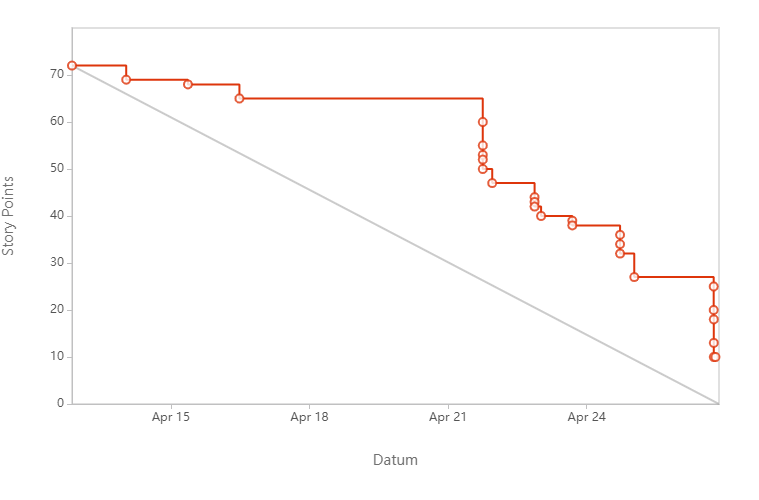
\includegraphics[width=0.5\textwidth]{Sprint_3_Burndown_Chart}
		\caption{Sprint 3 Burndown-Chart}
	\end{figure}



\end{document}